\section{Introduction}\label{sec:intro}

% Need a paragrapgh or two to explain why the tool is interesting and
% significant should be provided.

\dReach{} is a bounded model checker for hybrid systems. It encodes
bounded reachability problems of hybrid systems as first-order
formulas over the real numbers, and solves them using
$\delta$-decision procedures in the SMT solver \dReal{}. \dReach{} is
able to handle a wide range of highly nonlinear hybrid systems. It has
scaled well on various realistic nonlinear models from biomedical and
robotics applications~\cite{}.

It is well-known that the standard bounded reachability problems for
simple hybrid systems are already highly
undecidable~\cite{DBLP:conf/rex/AlurD91,DBLP:conf/hybrid/AlurCHH92}. In
previous work~\cite{}, we have defined the notion of
$\delta$-reachability problem of hybrid systems. In this new
framework, we have shown that bounded $\delta$-reachability is
decidable for a wide range of hybrid systems, with reasonable
complexity bounds~\cite{}. We give a brief review of the framework in
Section~\ref{sec:delta-reachability}.

Realistic hybrid systems involves nonlinear ODEs with transcendental
functions. \dReach{} allows users to specify a hybrid system in a
nonlinear signature as it is without linearizing or overapproximating
it. Users can provide the tool with a numerical error bound $\delta$,
a bounded time horizon $[0, T]$, and a maximum number of mode switches
$k$ for the analysis. As a result of analysis, \dReach{} will return
either \textbf{$\delta$-sat} with a concrete counterexample, or
\textbf{unsat} which does not involve numerical errors. We also
provide a visualization for the $\delta$-sat case to help
understand the analysis result.
\begin{figure}[!t]
  \subfloat[An example of nonlinear hybrid system model: off-treatment
  mode of the prostate cancer treatement model~\cite{}\label{subfig-1:prostate}]{
    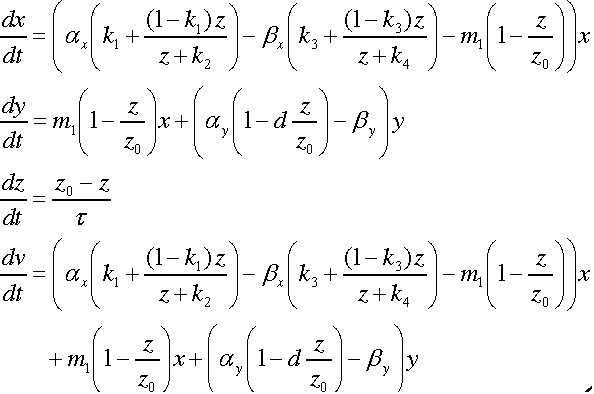
\includegraphics[width=0.48\textwidth]{images/prostatebw-mode2.pdf}
  }
  \hfill
  \subfloat[Visualization of a concrete counterexample generated from
  dReach for the prostate cancer treatment model.]{%
    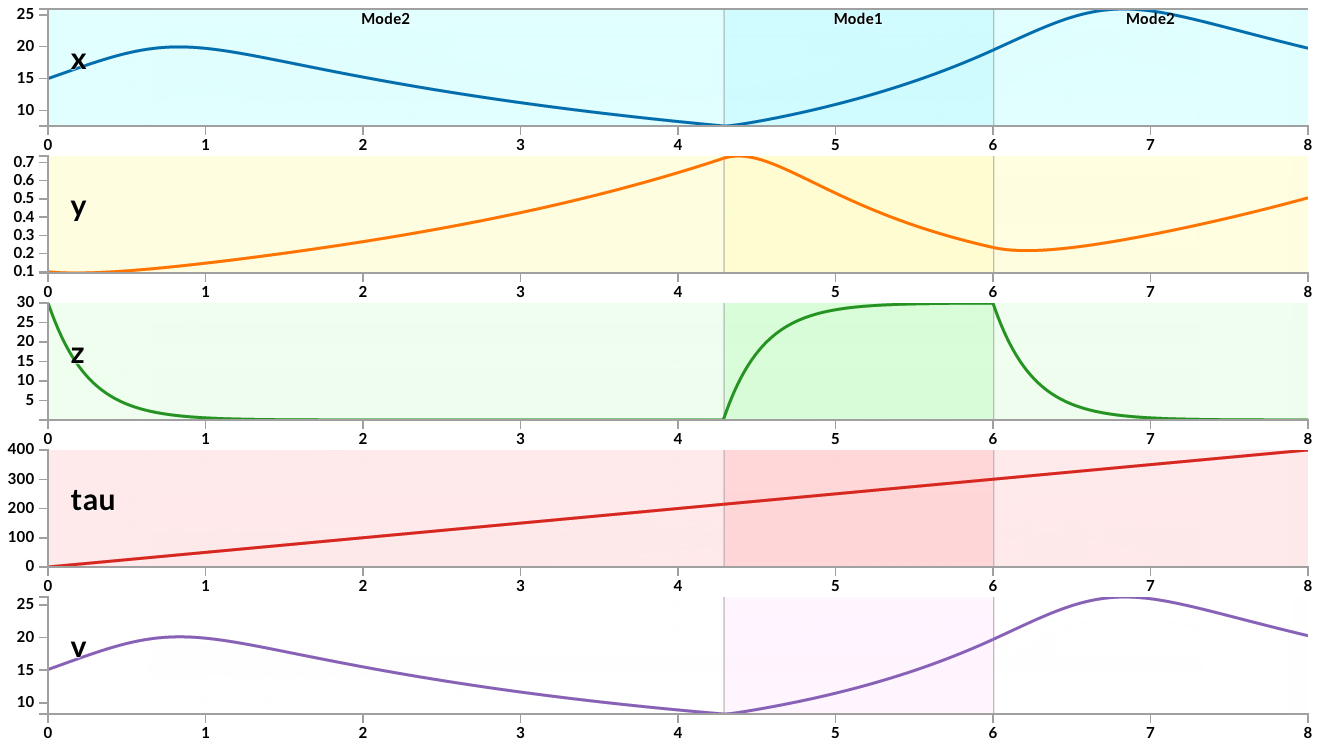
\includegraphics[width=0.48\textwidth]{images/prostate}
  }
  \caption{An example of nonlinear hybrid system model: Prostate
    cancer model.}
  \label{fig:prostate-example}
\end{figure}
For instance, figure~\ref{fig:prostate-example} shows a part of a
prostate cancer treatment model that contains nonlinear ODEs and a
visualization of a generated concrete counterexample.

\paragraph{Related Work}
%reachable set computation tools: flow star, SpaceX, Phaver,
%theorem provers:
%similar tools: iSAT, RSolver -- emphasize on the nonlinearity that we can handle.

The paper is structured as follows.


%%% Local Variables:
%%% mode: latex
%%% TeX-master: "main"
%%% End:
